
%(BEGIN_QUESTION)
% Copyright 2010, Tony R. Kuphaldt, released under the Creative Commons Attribution License (v 1.0)
% This means you may do almost anything with this work of mine, so long as you give me proper credit

A rock-crushing operation uses a set of water spray nozzles to ``knock down'' dust released by the rocks as they exit the crushing machine down a chute and onto a conveyor belt:

$$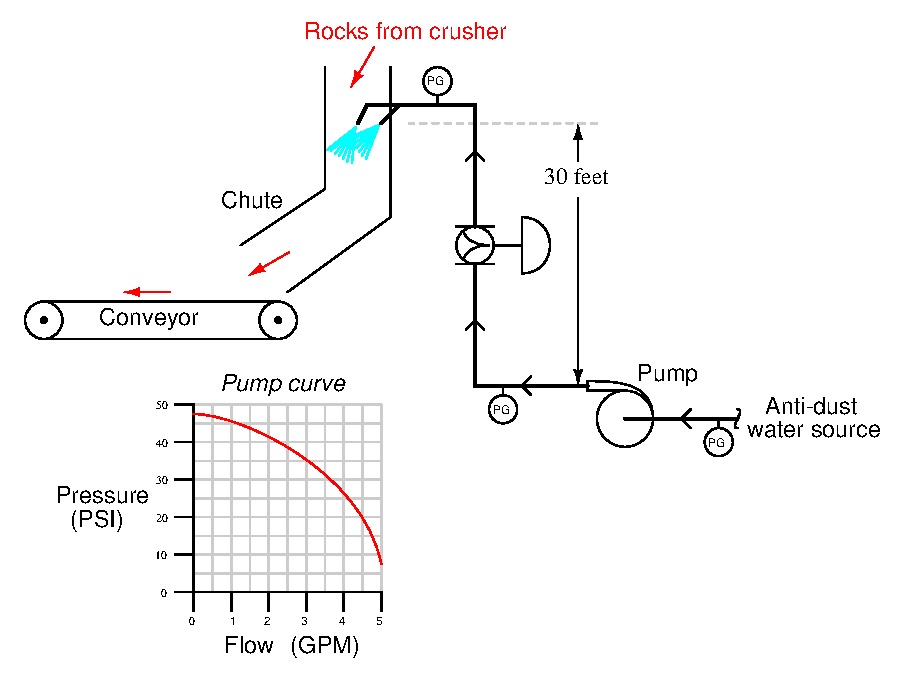
\includegraphics[width=15.5cm]{i01409x01.eps}$$

Determine the required $C_{v}$ rating for this control valve to provide a flow rate of 3 GPM, assuming the nozzles drop approximately 4 PSI of water pressure at that flow rate and that the pump suction (inlet) pressure is 0 PSIG at all times.

\vskip 10pt

Suppose an operator suspects the spray nozzles are plugged, and calls you to confirm this with some sort of diagnostic test.  Neither the spray nozzles nor the rocks falling through the chute are visible for inspection, since all this is enclosed for safety reasons, and the process must be kept running.  How is it possible for you to diagnose plugged nozzles from outside the chute?  Devise a test to confirm (or disprove) the operator's hypothesis.

\vskip 20pt \vbox{\hrule \hbox{\strut \vrule{} {\bf Suggestions for Socratic discussion} \vrule} \hrule}

\begin{itemize}
\item{} What type of control valve and actuator are used in this application?
\item{} Does it matter where the control valve is installed in the vertical pipe section (e.g. at the top versus at the bottom versus in the middle)?  Explain why or why not.
\item{} How do you think the pump curve would be affected if the pump's speed were altered (e.g. the AC electric motor powered through a VFD)?
\end{itemize}

\underbar{file i01409}
%(END_QUESTION)





%(BEGIN_ANSWER)

$C_{v}$ = 0.71
 
%(END_ANSWER)





%(BEGIN_NOTES)

$$\Delta P = 35 - \left(30 \hbox{ ft WC} \over 1 \right)  \left(12 \hbox{ in} \over 1 \hbox{ ft}\right)  \left(1 \hbox{ PSI} \over 27.68 \hbox{ "WC} \right) - 4 = 17.99 \hbox{ PSID}$$

$$Q = C_v \sqrt{\Delta P \over G_f}$$

$$C_v = {Q \over \sqrt{\Delta P \over G_f}}$$

$$C_v = {3 \over \sqrt{17.99 \over 1}} = 0.71$$


\vskip 10pt

Perhaps the simplest test is to observe the pressure gauge at the nozzle inlet pipe as the control valve is opened and closed.  Good nozzles will exhibit gauges pressures at that location varying between 0 PSI (no flow) and approximately 4 PSI (full flow).  Plugged nozzles will register significantly higher pressures than 4 PSI, and if severely plugged may not even return to 0 PSI when the control valve is fully shut.

%INDEX% Final Control Elements, pump: pressure/flow curve
%INDEX% Final Control Elements, valve: sizing

%(END_NOTES)


